\documentclass[25pt, a0paper, portrait, margin=0mm, innermargin=15mm,
     blockverticalspace=6mm, colspace=14mm, subcolspace=6mm]{tikzposter}

\usepackage[utf8]{inputenc}
\usepackage[T1]{fontenc}
\usepackage{lmodern}
\usepackage{amsmath, amssymb}
\usepackage{booktabs}
\usepackage{graphicx}
\usepackage{tikz}
\usepackage{xcolor}
\usepackage{array}
\usepackage{qrcode}
\usepackage{colortbl}
\usetikzlibrary{shapes, arrows.meta, positioning, fit, backgrounds, decorations.pathreplacing}

\definecolor{munavy}{HTML}{003C71}
\definecolor{muaccent}{HTML}{E74C3C}
\definecolor{mugreen}{HTML}{27AE60}
\definecolor{mubg}{HTML}{F4F6F8}
\definecolor{mugrey}{HTML}{6C757D}
\definecolor{muyellow}{HTML}{F1C40F}
\definecolor{muorange}{HTML}{E67E22}
\definecolor{mupurple}{HTML}{8E44AD}
\definecolor{muteal}{HTML}{16A085}

\definecolorstyle{murlStyle}{
    \definecolor{colorOne}{named}{munavy}
    \definecolor{colorTwo}{named}{mubg}
    \definecolor{colorThree}{named}{muaccent}
}{
    \colorlet{backgroundcolor}{white}
    \colorlet{framecolor}{munavy}
    \colorlet{titlefgcolor}{white}
    \colorlet{titlebgcolor}{munavy}
    \colorlet{blocktitlebgcolor}{munavy}
    \colorlet{blocktitlefgcolor}{white}
    \colorlet{blockbodybgcolor}{white}
    \colorlet{blockbodyfgcolor}{black}
    \colorlet{innerblocktitlebgcolor}{munavy}
    \colorlet{innerblocktitlefgcolor}{white}
    \colorlet{innerblockbodybgcolor}{mubg}
    \colorlet{innerblockbodyfgcolor}{black}
    \colorlet{notefgcolor}{black}
    \colorlet{notebgcolor}{mubg}
    \colorlet{noteframecolor}{munavy}
}

\usetheme{Default}
\usecolorstyle{murlStyle}
\useblockstyle{Default}
\usetitlestyle{Default}

\title{Learning When to Warn, When to Ban}
\author{Rishabh Jain}
\institute{Department of Computer Science, Maynooth University}

\settitle{
    \centering
    \vspace{1mm}
    {\fontsize{76}{86}\selectfont\bfseries\color{titlefgcolor} Learning When to Warn, When to Ban}\\[5mm]
    {\fontsize{42}{50}\selectfont\color{titlefgcolor} Constrained Reinforcement Learning for Multilingual Content Moderation}\\[5mm]
    {\fontsize{30}{36}\selectfont\color{titlefgcolor} \@author \quad$|$\quad \@institute \quad$|$\quad MURL 2026}
    \vspace{1mm}
}

\begin{document}
\tikzposterlatexaffectionproofoff
\maketitle[width=0.96\textwidth, titletotopverticalspace=6mm, titletoblockverticalspace=8mm]

% ============================================================
% ROW 1 : Problem + Contributions  (full width, two columns inside)
% ============================================================
\block{1. The Problem and Our Contributions}{
\large
\begin{minipage}[t]{0.48\linewidth}
\textbf{\Large The Problem.}\\[1mm]

Automated content moderation on multilingual platforms like Discord is broken in following ways:\\[2mm]
\begin{itemize}\setlength\itemsep{1mm}
    \item \textbf{No user history:} Every message is scored in isolation, a user who sends ten borderline messages in a row gets the same response as a first-time offender, because the system has no memory of prior behavior.
    \item \textbf{Binary decisions only:} The output is always either remove or permit, there is no mechanism to issue a warning, temporarily suspend, or escalate gradually, so the system cannot mirror the nuanced enforcement humans apply.
\end{itemize}\\[2mm]


\end{minipage}\hfill
\vrule width 0.5pt\hfill
\begin{minipage}[t]{0.48\linewidth}
\textbf{\Large Four Contributions.}\\[1mm]
\begin{itemize}\setlength\itemsep{1mm}
    \item \textbf{CMDP framing} of moderation with a 5-level escalation ladder and constraint costs for fairness.
    \item \textbf{Hard action masking} enforces procedural escalation at the policy distribution, not in the reward.
    \item \textbf{Per-language affine calibration} of XLM-R scores neutralises classifier bias before it reaches the policy.
    \item \textbf{Dual fairness protection}: adaptive Lagrangian + Disparate Impact wrapper, both training-time.
\end{itemize}
\end{minipage}
}

% ============================================================
% ROW 2 : The CMDP and Action Ladder  (full width)
% ============================================================
\block{2. Moderation as a Constrained Markov Decision Process}{
\large
We solve $\mathcal{M} = \langle S, A, P, R, \mathbf{C}, \mathbf{d}, \gamma\rangle$ via Lagrangian relaxation:
$\;\max_\pi V_R^\pi$ subject to $V_{C_k}^\pi \leq d_k$ for all constraints $k$ (false-positive rate, per-language ban-rate parity).\\[3mm]

\begin{center}
\begin{tikzpicture}[node distance=18mm, font=\large\bfseries]
\node[draw, rounded corners, fill=mugreen!35,              minimum width=78mm, minimum height=22mm] (a) {ALLOW};
\node[draw, rounded corners, fill=muyellow!50,             minimum width=78mm, minimum height=22mm, right=of a] (w) {WARN};
\node[draw, rounded corners, fill=muorange!55,             minimum width=78mm, minimum height=22mm, right=of w] (d) {DELETE};
\node[draw, rounded corners, fill=muaccent!55,             minimum width=78mm, minimum height=22mm, right=of d] (t) {TIMEOUT};
\node[draw, rounded corners, fill=muaccent!85, minimum width=78mm, minimum height=22mm, right=of t] (b) {BAN};
\node[font=\footnotesize\mdseries, below=1mm of a] {$s_t < 0.85$};
\node[font=\footnotesize\mdseries, below=1mm of w] {$s_t \geq 0.15$};
\node[font=\footnotesize\mdseries, below=1mm of d] {$s_t \geq 0.15$};
\node[font=\footnotesize\mdseries, below=1mm of t] {$s_t{\geq}0.15,\,e_t{\geq}2$};
\node[font=\footnotesize\mdseries, below=1mm of b] {prior TIMEOUT};
\draw[-{Stealth[length=5mm]}, ultra thick, munavy] (a) -- (w);
\draw[-{Stealth[length=5mm]}, ultra thick, munavy] (w) -- (d);
\draw[-{Stealth[length=5mm]}, ultra thick, munavy] (d) -- (t);
\draw[-{Stealth[length=5mm]}, ultra thick, munavy] (t) -- (b);
\end{tikzpicture}
\end{center}

\vspace{2mm}
\begin{minipage}[t]{0.32\linewidth}
\centering
\colorbox{munavy}{\parbox{0.95\linewidth}{\centering\color{white}\vspace{1mm}\textbf{\large Single Multilingual Policy}\vspace{1mm}}}\\[2mm]
\normalsize One MaskablePPO network across 13 languages fairness comparisons \textit{across} languages become coherent because the same policy is evaluated.
\end{minipage}\hfill
\begin{minipage}[t]{0.32\linewidth}
\centering
\colorbox{muaccent}{\parbox{0.95\linewidth}{\centering\color{white}\vspace{1mm}\textbf{\large Hard Procedural Masking}\vspace{1mm}}}\\[2mm]
\normalsize Mask $\mathbf{m}_t \in \{0,1\}^5$ removes illegal actions from the policy distribution \textit{before} sampling a learned policy cannot propose them even by accident.
\end{minipage}\hfill
\begin{minipage}[t]{0.32\linewidth}
\centering
\colorbox{mugreen}{\parbox{0.95\linewidth}{\centering\color{white}\vspace{1mm}\textbf{\large Fairness in the Loss}\vspace{1mm}}}\\[2mm]
\normalsize $\lambda_{k+1} = \max(\epsilon,\lambda_k+\alpha_\lambda(\hat{V}_{C_k}-d_k))$ adaptive multiplier on FP rate; Disparate Impact wrapper penalises any language $> 1.5\times$ baseline.
\end{minipage}
}

% ============================================================
% ROW 3 : Architecture (left) | Headline Result (right)
% ============================================================
\begin{columns}

\column{0.5}
\block{3. System Architecture}{
\large
\begin{center}
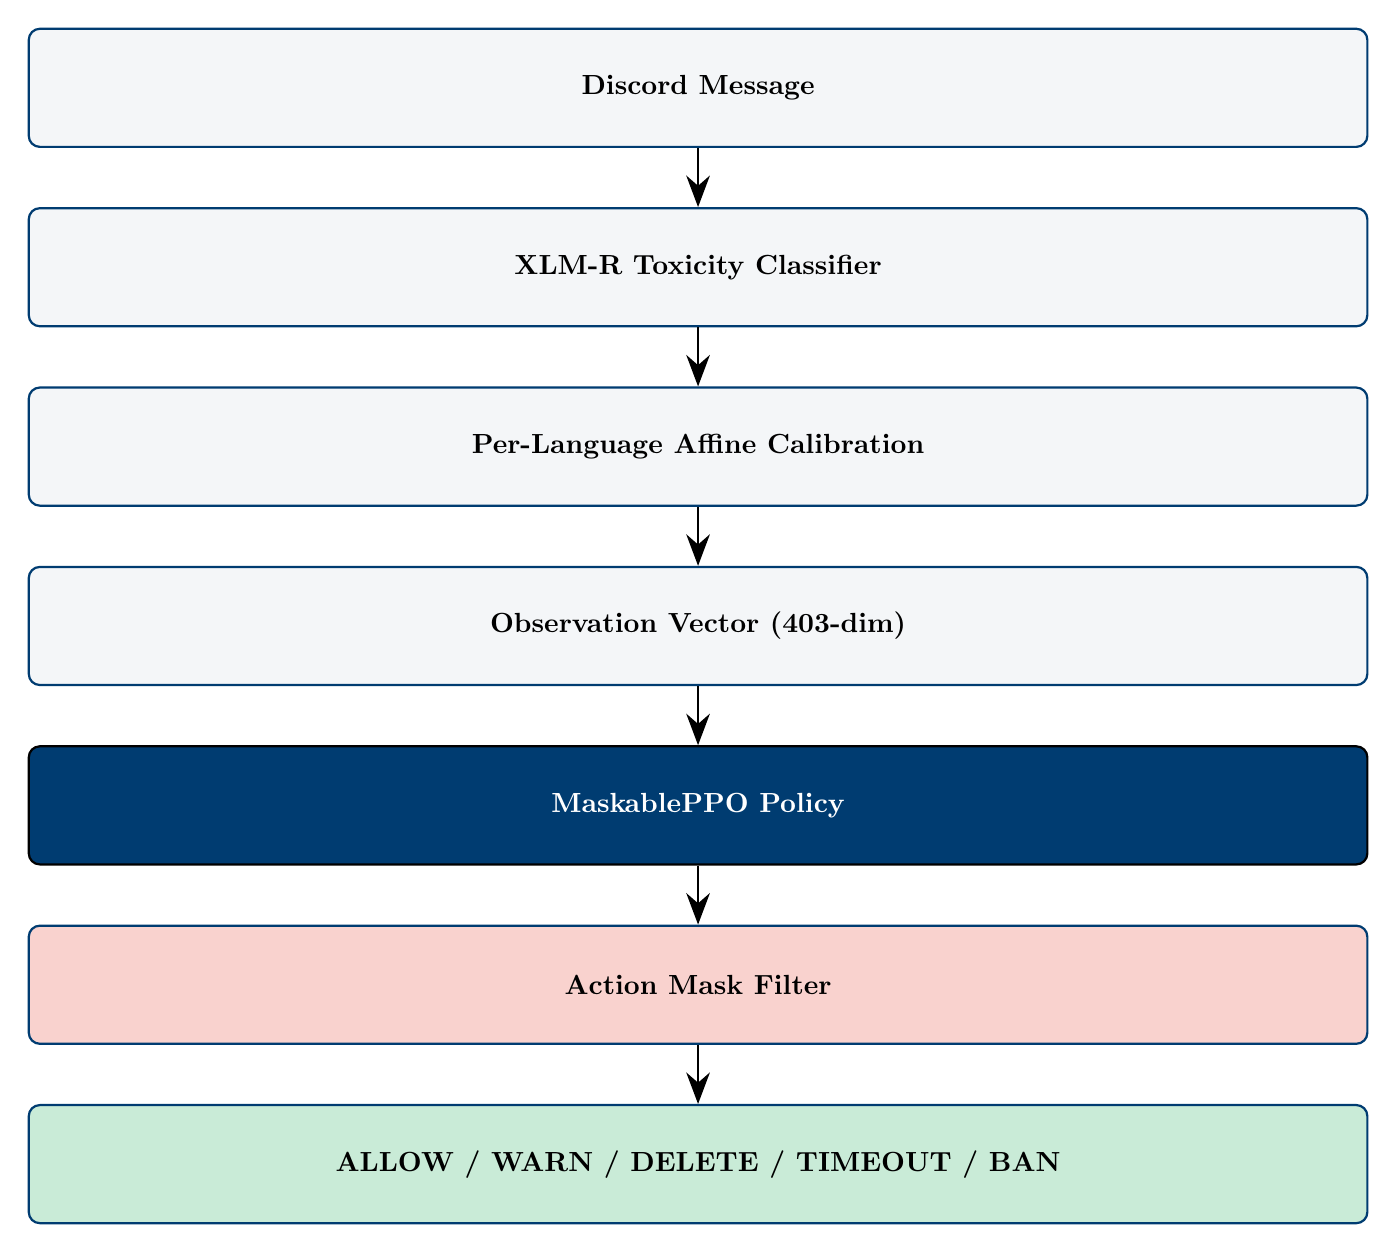
\begin{tikzpicture}[
    node distance=7.5mm, font=\normalsize\bfseries,
    box/.style={draw, rounded corners, fill=mubg, minimum width=170mm,
                minimum height=15mm, align=center, thick, draw=munavy},
    accent/.style={draw, rounded corners, fill=munavy, text=white,
                minimum width=170mm, minimum height=15mm, align=center, thick}
]
\node[box] (msg)  {Discord Message};
\node[box, below=of msg]  (xlmr) {XLM-R Toxicity Classifier};
\node[box, below=of xlmr] (cal)  {Per-Language Affine Calibration};
\node[box, below=of cal]  (obs)  {Observation Vector (403-dim)};
\node[accent, below=of obs]        (ppo)  {MaskablePPO Policy};
\node[box, below=of ppo,  fill=muaccent!25] (mask) {Action Mask Filter};
\node[box, below=of mask, fill=mugreen!25]  (act)  {ALLOW / WARN / DELETE / TIMEOUT / BAN};
\foreach \a/\b in {msg/xlmr,xlmr/cal,cal/obs,obs/ppo,ppo/mask,mask/act}
    \draw[-{Stealth[length=4mm]}, thick] (\a)--(\b);
\end{tikzpicture}
\end{center}

\vspace{2mm}
{\colorlet{innerblocktitlebgcolor}{muaccent}
\innerblock{Hard Action-Masking Rules}{
\normalsize
\begin{itemize}\setlength\itemsep{1mm}
    \item \textbf{BAN} requires a prior TIMEOUT in the user's history
    \item \textbf{TIMEOUT} requires $\geq 2$ prior infractions
    \item \textbf{Punitive actions} blocked when toxicity score $< 0.15$
    \item \textbf{ALLOW} blocked when toxicity score $\geq 0.85$
\end{itemize}
}}
\vspace{2mm}
}

\column{0.5}
\block{5. Headline Result}{
\large
\begin{center}
\renewcommand{\arraystretch}{1.5}
\setlength{\tabcolsep}{8pt}
\begin{tabular}{lcccc}
\toprule
\textbf{System} & \textbf{Acc.} & \textbf{FP} & \textbf{FN} & \textbf{TIME/BAN} \\
\midrule
Keyword filter   & 0.673 & 0.020 & 0.272 & {\color{muaccent}\textbf{$\times$}} \\
Static threshold & 0.720 & 0.190 & 0.250 & {\color{muaccent}\textbf{$\times$}} \\
\rowcolor{mubg}\textbf{RL agent} & \textbf{0.736} & 0.153 & 0.0001 & {\color{mugreen}\textbf{\checkmark}} \\
\bottomrule
\end{tabular}
\end{center}

\vspace{2mm}
\begin{center}
\colorbox{muaccent}{\parbox{0.94\linewidth}{\centering\color{white}\bfseries
\vspace{3mm}\large
The only system tested that correctly issues TIMEOUT and BAN
\vspace{5mm}}}
\end{center}

\vspace{3mm}
\textbf{Per-class accuracy on held-out test split (8{,}016 steps):}\\[1mm]
\begin{center}
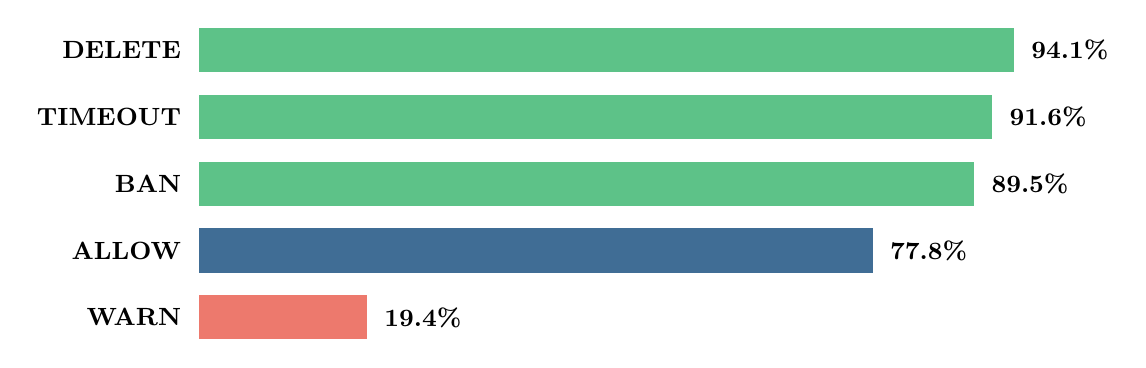
\begin{tikzpicture}[font=\small, x=1cm, y=1cm]
\foreach \lbl/\val/\col [count=\i] in {%
    DELETE/94.1/mugreen,
    TIMEOUT/91.6/mugreen,
    BAN/89.5/mugreen,
    ALLOW/77.8/munavy,
    WARN/19.4/muaccent}
{
    \node[anchor=east, font=\small\bfseries] at (2.0, -\i*0.85) {\lbl};
    \fill[\col!75] (2.1, -\i*0.85-0.28) rectangle ({2.1 + \val/100 * 11}, -\i*0.85+0.28);
    \node[anchor=west, font=\small\bfseries] at ({2.2 + \val/100 * 11}, -\i*0.85) {\val\%};
}
\end{tikzpicture}
\end{center}

\vspace{1mm}
{\colorlet{innerblocktitlebgcolor}{mugreen}
\innerblock{Why the RL Agent Wins}{
\footnotesize
Static baselines have \textit{no notion of user history}, so they can never reach TIMEOUT or BAN.
The RL agent's elevated FP (0.153) is dominated by WARN-on-benign strictly lower-harm than false DELETE/BAN.
}}
}

\end{columns}

% ============================================================
% ROW 4 : Two-Stage Training (left) | Fairness Audit (right)
% ============================================================
\begin{columns}

\column{0.5}
\block{4. Two-Stage Training}{
\large
\begin{center}
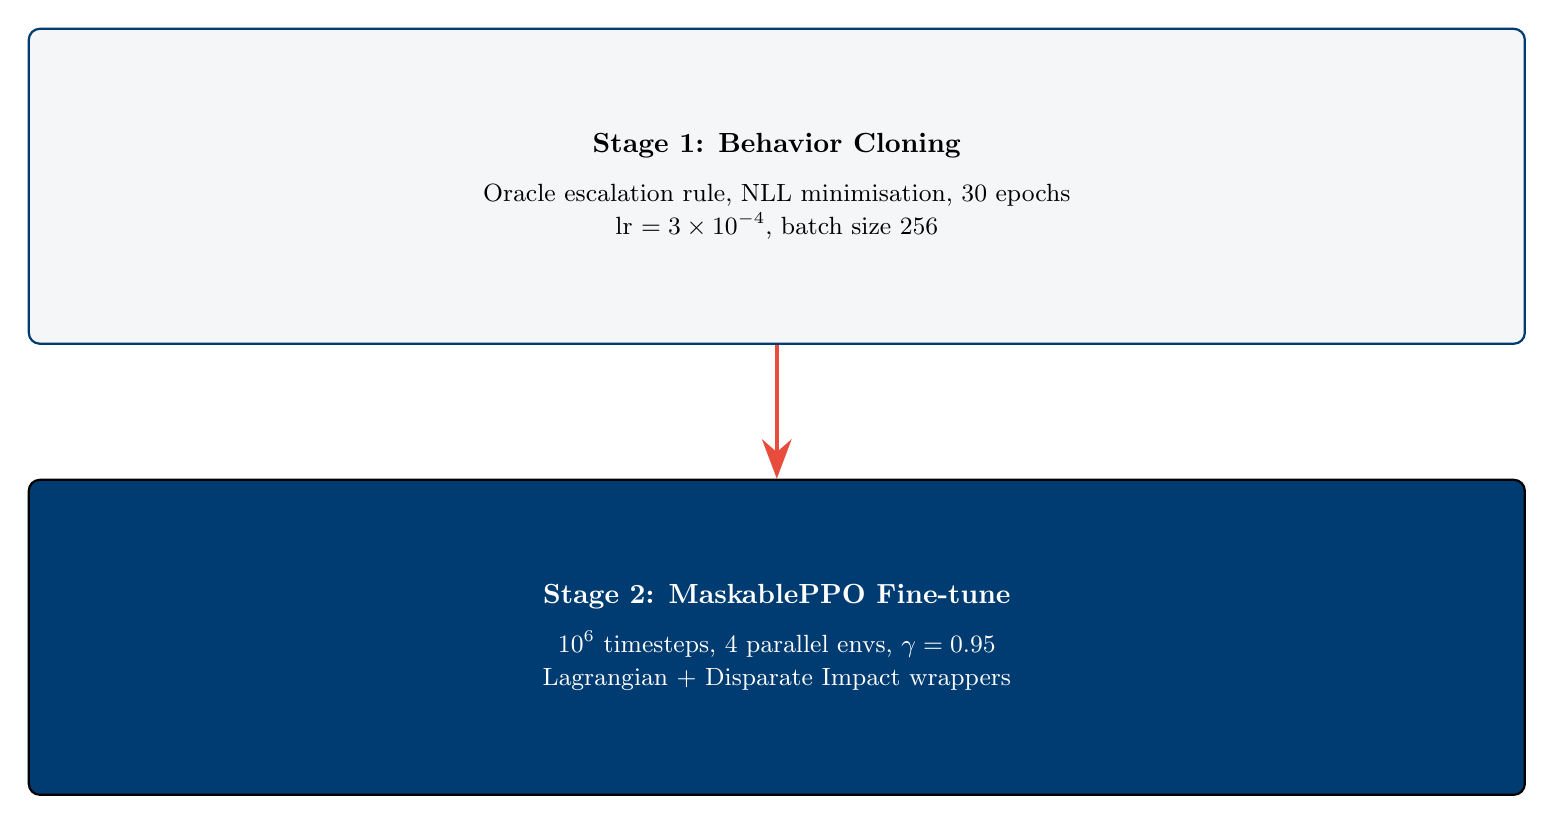
\begin{tikzpicture}[font=\normalsize\bfseries, node distance=17mm]
\node[draw, rounded corners, fill=mubg, thick, draw=munavy,
      minimum width=190mm, minimum height=40mm, align=center] (bc)
      {Stage 1: Behavior Cloning\\[2mm]
       \small\mdseries Oracle escalation rule, NLL minimisation, 30 epochs\\
       \small\mdseries lr $= 3\times10^{-4}$, batch size 256};
\node[draw, rounded corners, fill=munavy, text=white, thick,
      minimum width=190mm, minimum height=40mm, align=center, below=of bc] (rl)
      {Stage 2: MaskablePPO Fine-tune\\[2mm]
       \small\mdseries $10^6$ timesteps, 4 parallel envs, $\gamma = 0.95$\\
       \small\mdseries Lagrangian + Disparate Impact wrappers};
\draw[-{Stealth[length=5mm]}, ultra thick, muaccent] (bc) -- (rl);
\end{tikzpicture}
\end{center}

\vspace{6mm}
{\colorlet{innerblocktitlebgcolor}{muorange}
\innerblock{Synthetic Data Pipeline}{
\normalsize
\textbf{595 episodes} (8{,}016 steps) across \textbf{14 language categories}.
Generated via DeepSeek V3.1 from Jigsaw + textdetox seeds, $k$-means clustered.
80/20 split. Mix: 30\% toxic / 25\% benign / 20\% escalating / 15\% mild / 10\% subtle.
}}
\vspace{6mm}
}

\column{0.5}
\block{6. Cross-Lingual Fairness Audit}{
\large
Per-language BAN rate vs.\ the $1.5\times$ parity threshold:\\[2mm]

\vspace{-17mm}

\begin{center}
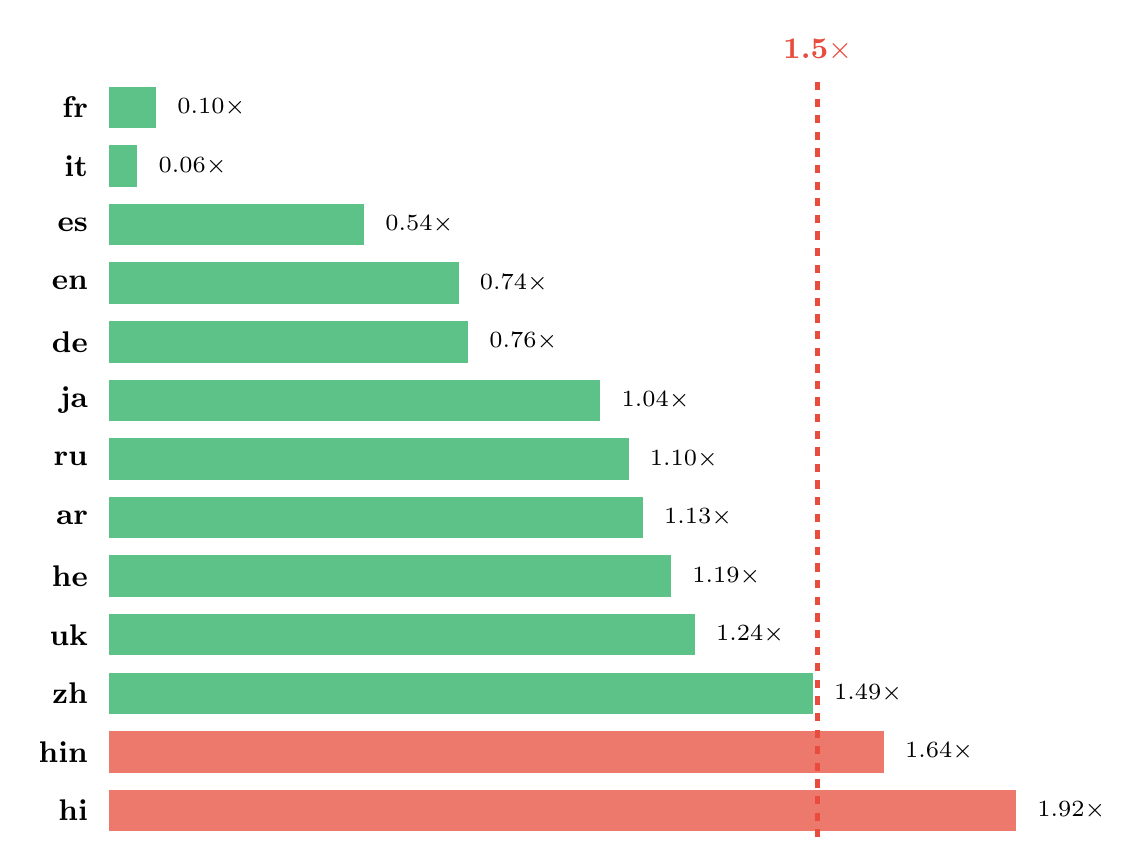
\begin{tikzpicture}[font=\small, x=1cm, y=1cm, scale=1.2, transform shape]
\foreach \lang/\ratio/\col [count=\i] in {%
    fr/0.10/mugreen, it/0.06/mugreen, es/0.54/mugreen,
    en/0.74/mugreen, de/0.76/mugreen, ja/1.04/mugreen,
    ru/1.10/mugreen, ar/1.13/mugreen, he/1.19/mugreen,
    uk/1.24/mugreen, zh/1.49/mugreen,
    hin/1.64/muaccent, hi/1.92/muaccent}
{
    \node[anchor=east, font=\small\bfseries] at (1.8, -\i*0.62) {\lang};
    \fill[\col!75] (1.9, -\i*0.62-0.22) rectangle ({1.9 + \ratio*5}, -\i*0.62+0.22);
    \node[anchor=west, font=\scriptsize] at ({2.0 + \ratio*5}, -\i*0.62) {\ratio$\times$};
}
\draw[muaccent, ultra thick, dashed] (1.9 + 1.5*5, -0.35) -- (1.9 + 1.5*5, -8.35);
\node[muaccent, font=\small\bfseries, anchor=south] at (1.9 + 1.5*5, -0.25) {1.5$\times$};
\end{tikzpicture}
\end{center}

{\colorlet{innerblocktitlebgcolor}{mugreen}
\innerblock{Diagnosis: Model Bias, Not Policy Bias}{
\normalsize
\textbf{12 of 14 categories pass parity.} Hindi ($1.92\times$) and Hinglish
($1.64\times$) gaps trace to upstream XLM-R bias ($+0.095$ over English).
Calibration cannot fix this $\Rightarrow$ \textit{recommend classifier fine-tuning}.
}}
\vspace{2mm}
}

\end{columns}

% ============================================================
% ROW 5 : Key Takeaways  (full width)
% ============================================================
\begin{columns}
\column{1}
\block{Key Takeaways}{
\large
\begin{itemize}\setlength\itemsep{2mm}
    \item \textbf{Action masking} provides hard procedural guarantees that
          reward shaping alone cannot match a learned policy literally
          cannot propose an illegal escalation.
    \item \textbf{Fairness as a training-time objective} (Lagrangian +
          Disparate Impact wrapper) cleanly isolates \textit{policy bias}
          from \textit{model bias}, pointing remediation at the right
          component.
    \item \textbf{Synthetic-data RL with two-stage BC$\to$PPO} reaches
          actions that static baselines fundamentally cannot produce the
          only system tested with correct TIMEOUT and BAN behaviour.
\end{itemize}
}
\end{columns}

% ============================================================
% ROW 6 : By the Numbers  (full width, colourful stat boxes)
% ============================================================
\begin{columns}
\column{1}
\block{}{%
\newcommand{\stathex}[3]{%
    \begin{minipage}[c]{0.18\linewidth}
    \centering
    \fcolorbox{#1}{#1}{%
        \begin{minipage}[c]{0.93\linewidth}
        \centering\color{white}
        \vspace{4mm}
        {\bfseries\Large #2}\\[2mm]
        {\bfseries\large #3}
        \vspace{2mm}
        \end{minipage}%
    }
    \end{minipage}%
}
\noindent\begin{minipage}{\linewidth}
\centering
\stathex{munavy}{13}{Languages covered}\hfill
\stathex{mugreen}{91.7\%}{Accuracy on Actions}\hfill
\stathex{muorange}{12/14}{Fairness categories pass}\hfill
\stathex{muaccent}{$10^{-4}$}{False-negative rate}\hfill
\stathex{mupurple}{595}{Synthetic episodes}
\end{minipage}
}
\end{columns}

\end{document}
